% Fig. 2 -- IG-DCTF system architecture (full width, 7.16 in).
% Compile with pdfLaTeX (Overleaf default). Output: fig02_architecture.pdf
\documentclass[border=3pt]{standalone}
\usepackage[T1]{fontenc}
\usepackage{newtxtext,newtxmath}
\usepackage{tikz}
\usetikzlibrary{arrows.meta,positioning,calc}

\definecolor{acc}{RGB}{31,78,121}
\colorlet{accfill}{acc!10}
\colorlet{gfill}{black!7}

\tikzset{
  >={Stealth[length=3pt,width=2.6pt]},
  every node/.style={font=\footnotesize},
  blk/.style={draw=black,line width=0.5pt,fill=white,align=center,inner sep=2pt,minimum height=24pt},
  inp/.style={blk,fill=gfill,minimum width=88pt},
  chan/.style={blk,minimum width=56pt},
  outp/.style={blk,minimum width=104pt},
  accblk/.style={draw=acc,fill=accfill,line width=0.7pt},
  grpbox/.style={draw=black!60,line width=0.5pt,dash pattern=on 2.5pt off 2pt},
  accgrpbox/.style={draw=acc,line width=0.5pt,dash pattern=on 2.5pt off 2pt},
  flow/.style={->,line width=0.5pt},
  ftitle/.style={anchor=south west,inner sep=1pt,font=\footnotesize\bfseries},
}

\begin{document}
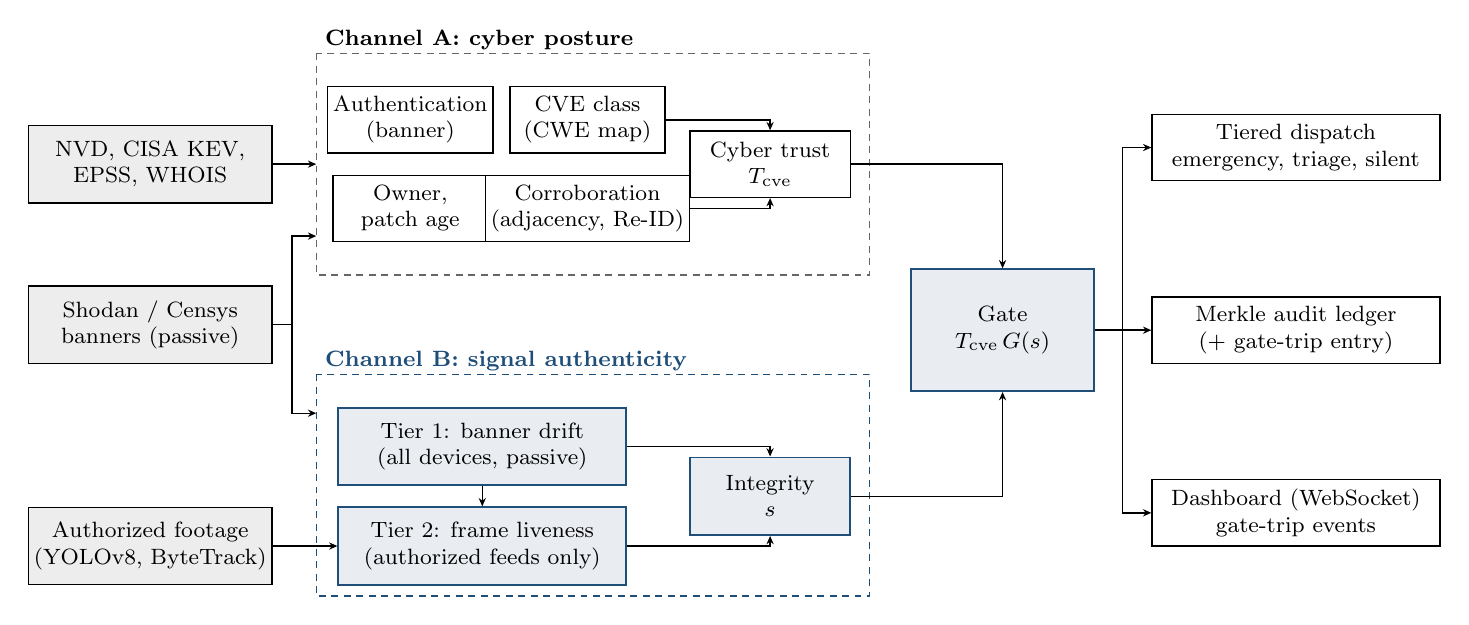
\begin{tikzpicture}[x=1pt,y=1pt]

  % ---------------- inputs
  \node[inp,minimum height=28pt] (inNVD)  at (48,-46)  {NVD, CISA KEV,\\EPSS, WHOIS};
  \node[inp,minimum height=28pt] (inSho)  at (48,-104) {Shodan / Censys\\banners (passive)};
  \node[inp,minimum height=28pt] (inVid)  at (48,-184) {Authorized footage\\(YOLOv8, ByteTrack)};

  % ---------------- Channel A
  \draw[grpbox] (108,-6) rectangle (308,-86);
  \node[ftitle] at (110,-6) {Channel A: cyber posture};
  \node[chan] (A1) at (142,-30) {Authentication\\(banner)};
  \node[chan] (A2) at (206,-30) {CVE class\\(CWE map)};
  \node[chan] (A3) at (142,-62) {Owner,\\patch age};
  \node[chan] (A4) at (206,-62) {Corroboration\\(adjacency, Re-ID)};
  \node[blk,minimum width=58pt] (Tc) at (272,-46) {Cyber trust\\$T_{\mathrm{cve}}$};
  \draw[flow] (A2.east) -| (Tc.north);
  \draw[flow] (A4.east) -| (Tc.south);

  % ---------------- Channel B
  \draw[accgrpbox] (108,-122) rectangle (308,-202);
  \node[ftitle,text=acc] at (110,-122) {Channel B: signal authenticity};
  \node[chan,accblk,minimum width=104pt,minimum height=28pt] (B1) at (168,-148) {Tier 1: banner drift\\(all devices, passive)};
  \node[chan,accblk,minimum width=104pt,minimum height=28pt] (B2) at (168,-184) {Tier 2: frame liveness\\(authorized feeds only)};
  \node[blk,accblk,minimum width=58pt,minimum height=28pt] (Sg) at (272,-166) {Integrity\\$s$};
  \draw[flow] (B1.east) -| (Sg.north);
  \draw[flow] (B2.east) -| (Sg.south);
  \draw[flow] (B1.south) -- (B2.north);

  % ---------------- gate
  \node[blk,accblk,minimum width=66pt,minimum height=44pt] (G) at (356,-106) {Gate\\$T_{\mathrm{cve}}\,G(s)$};
  \draw[flow] (Tc.east) -| (G.north);
  \draw[flow] (Sg.east) -| (G.south);

  % ---------------- outputs
  \node[outp] (O1) at (462,-40)  {Tiered dispatch\\emergency, triage, silent};
  \node[outp] (O2) at (462,-106) {Merkle audit ledger\\(+ gate-trip entry)};
  \node[outp] (O3) at (462,-172) {Dashboard (WebSocket)\\gate-trip events};
  \draw[flow] (G.east) -- (O2.west);
  \draw[flow] (G.east) -- ++(10,0) |- (O1.west);
  \draw[flow] (G.east) -- ++(10,0) |- (O3.west);

  % ---------------- inputs -> channels
  \draw[flow] (inNVD.east) -- (108,-46);
  \draw[flow] (inSho.east) -- ++(7,0) |- (108,-72);
  \draw[flow] (inSho.east) -- ++(7,0) |- (108,-136);
  \draw[flow] (inVid.east) -- (B2.west);
\end{tikzpicture}
\end{document}
